\documentclass[a4paper]{article}
\usepackage{float}
\usepackage{dsfont}
\usepackage{tipa}
\usepackage{amsmath}
\usepackage[english]{babel}
\usepackage[utf8]{inputenc}
\usepackage{amsmath}
\usepackage{graphicx}
\usepackage{caption}
\usepackage[colorinlistoftodos]{todonotes}

\DeclareMathOperator*{\argmin}{arg\,min} 

\title{CS5785 Applied Machine Learning}

\author{Prof Nathan Kallus, Cornell Tech\\
		Scribe: Celi Sun, Kang Raye Ng, Nian Ji,\\
        Sophie Fang, Yu Jin Hur}

\date{Sept. 11, 2018}

\begin{document}
\maketitle

\section{The Basis-Variance Trade-off}
A supervised learning algorithm can be understood as a function \textit{A} from data D = \{$X_{1}$,$Y_{1}$...,$X_{n}$,$Y_{n}$\} to a prediction rule $\hat{f}$:

\begin{center}
					$\hat{f} = \textit{A}(\textit{D})$
\end{center}

\noindent An algorithm is a general procedure, applied to any recurring dataset. Hence, a good algorithm is one that does well overall, i.e. should have a small average loss, \textit{R}(\textit{A}).

\begin{align*}
     R(A) &=E_D[R(A(D))]\\ 
     &=E_D[R(\hat{f})]\\
     &=E_D[E_x,_y\{l(Y, \hat{f}(x))\}]\\
     &=E_D[E_x,_y\{(\hat{f}(X)-Y)^2\}]\\   
	 \\
     R(\hat{f}(X)) &=E_x,_y[(\hat{f}(X)-Y)^2]\\ 
     &=E_x[E_y[(\hat{f}(X)-Y)^2|X]\\
     &=E_x[(\hat{f}(X)^2-2\hat{f}(X)E[Y|X]+E[Y^2|X]]\\
     &=E_x[\hat{f}(X)^2-2f(X)f^*(X)+f^*(X)^2-f^*(X)^2+E[Y^2|X]\\
     &=E_x[(\hat{f}(X)-f^*(X))^2]+E_x[Var(Y|X)]\\
	 \\
	 R(A) &=E_D[R\hat(f)]\\ 
     &=E_x[E_D[\hat(f)-f^*(x))^2]]+E_x[Var(Y|X)]\\
\end{align*}

\begin{align*}
	Err(X) &=E_D[(\hat{f}(X)-f^*(X))^2]\\ 
    &=E_D[([\hat{f}(X)-E_D(\hat{f}(X))]+[E_D(\hat{f}(X)-f^*(X)])^2]\\
    &=E_D[(\hat{f}(X)-E_D(\hat{f}(X)))^2]+[E_D(\hat{f}(X)-f^*(X)]^2\\
    &  +2E_D[\hat{f}(X)-E_D(\hat{f}(X))][E_D(\hat{f}(X))-f^*(X)]\\
    &=Var(\hat{f}(X))+[E_D(\hat{f}(X)-f^*(X)]^2\\
    &=Var(\hat{f}(X))+Bias(\hat{f}(X))^2\\
     \\
    R(A) &= Reducible Error + Irreducible Error\\
    &=E_X[Err(X)]+E_X[Var(Y|X)]\\
    &=Var(\hat{f}(X))+Bias(\hat{f}(X))^2+\sigma^2\\
\end{align*}

\noindent Based on the final result above, it can be shown that the average loss is a function of a reducible error (combination of variance and bias of algorithm) and irreducible error (variance of Y with respect to X). \\
\\
As such, an algorithm can be optimized by minimizing the reducible error by doing a trade-off between bias and variance as shown in figure 1 below. Intuitively, a model with a high complexity would tend to over-fit the data set resulting in an algorithm of low bias but high variance. In contrast, a model with low complexity would under-fit the data set resulting in an algorithm to have a low variance but high bias. 
\begin{figure}[H]
\centering
\captionsetup{justification=centering}
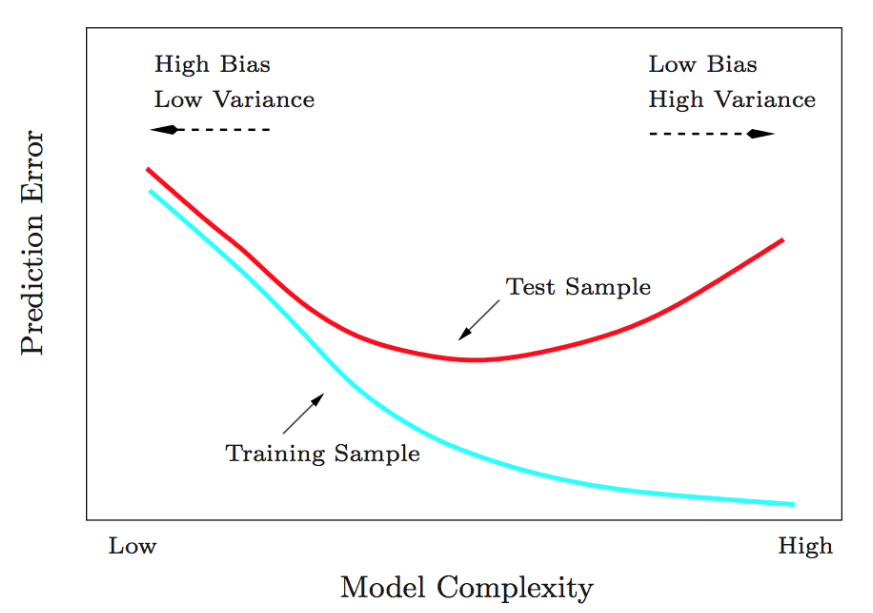
\includegraphics[width=1\textwidth]{Figure_1.PNG}
\caption{\label{fig:1}Test and training error as a function of model complexity.}
\end{figure}

\label{sec:tradeoff}

\section{Subset Selection}
Subset selection refers to the process of reducing model complexity to find a subset of features, X, that predict output,Y, well. The reasons for doing subset selection are as follows:
\begin{itemize}
  \item Reduce model complexity to avoid over-fitting.
  \item Allows for better trade-off between bias and variance
  \item Aids in interpretation to find important features that affect Y
\end{itemize}
Consider a linear regression model, $\hat{f}$, trained with ordinary least square (OLS) errors with data $D = \{X_1,Y_1,X_2,Y_2,...,X_n,Y_n\}$
\begin{align*}
	&\hat{f}(X)=X\beta, \quad \beta \in \mathds{R}^{1+p}\\
    &where\quad\beta_0 - intercept;\qquad \beta_{1:p} - coefficients 
\end{align*}
We introduce the support function which takes an input vector to output the index of non-zero entries. Applying the support function to \textbeta\ allows us to get a lower bound on the size of the minimum subset required. Note that the intercept is excluded from this selection.
\begin{align*}
	supp(\beta) = \{j = 1,2,...,p:\beta_j\neq 0\}
\end{align*}
Next the best-k features subset is selected based on evaluating the argmin function applied on the prediction error as shown below. Note that the best p feature coefficient is given by evaluating the data for linear regression with an OLS loss function.
\begin{align*}
	\hat{\beta}_{best-k} &= \argmin_{|supp(\beta)|\leq k}||Y-X\beta ||^2_2\\
    \hat{\beta}_{best-p} &= \hat{\beta}_{OLS}
\end{align*}
When p and k are large, the argmin function is difficult to compute manually as the possible permutations of picking k from p increases disproportionately as shown below.
$${p\choose k}\approx (\frac{p}{k})^k$$
Due to this complexity, there must be algorithms that facilitate the adding/removing of features to arrive at the best-k coefficients without manually computing every possibility. This can be achieved by comparing the absolute value of the coefficients, coefficients with larger values are thought to be more "influential". However this comparison is subject to scaling/normalization to a Z statistic. $Z_j$ refers to the normalized Z-statistic derived from the value of coefficient $\beta_j$.
\begin{align*}
    Z_j &= \frac{\hat{\beta_j}}{\hat{\sigma}\sqrt{v_j}}\\
    where \quad \hat{\sigma}=\frac{1}{n-k-1}&\sum_{i=1}^{n}{(Y_i-\hat{Y}_i)^2};\qquad 
    v_j=((X^TX)^{-1})_{jj}
\end{align*}
Based on the normalized coefficients/Z-score, we can follow the general rule to consider $\beta_j$ to be significant (at the p=0.05 level) if $|Z_j|\geq2$.\\
\\
Figure 2 shows how decreasing the model complexity/subset size from a large number, based on the Z-score of the coefficients, affects the training loss/residual sum-of-squares. It is shown that a subset size of 3 has almost the same training loss as a subset size of 8, despite having a significantly lower model complexity.

\begin{figure}[H]
\centering
\captionsetup{justification=centering}
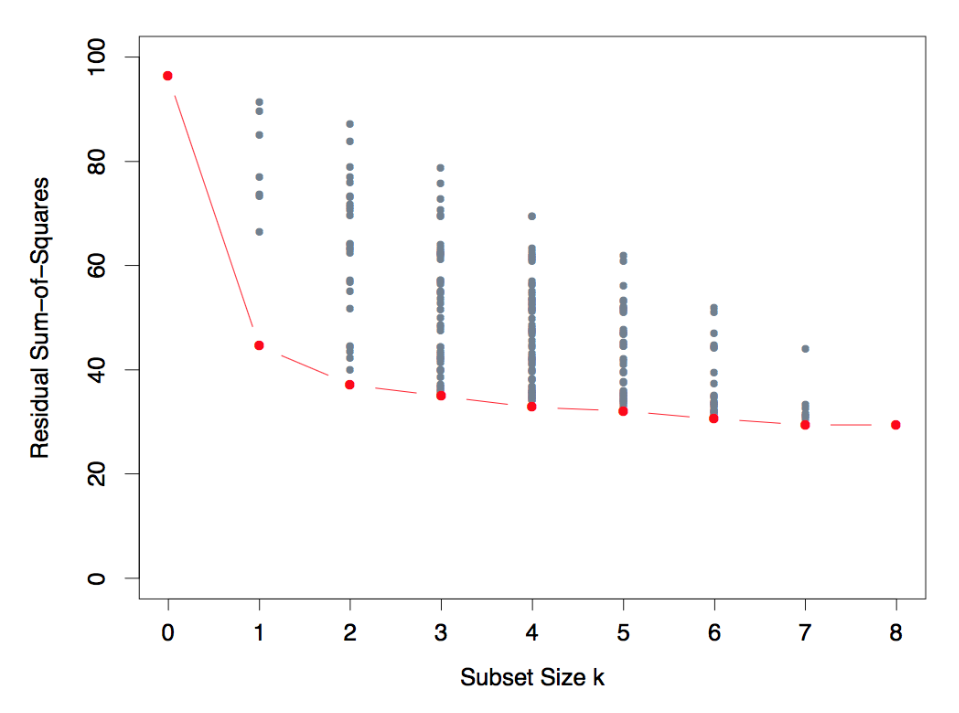
\includegraphics[width=1\textwidth]{Figure_2.PNG}
\caption{\label{fig:2}Residual Sum-of-Squares error for increasing subset size, k, for the prostate cancer example in the slides.}
\end{figure}

\label{sec:subset}

\noindent Next we look at 2 algorithms that can be used to do subset selection and reduce the complexity of a regression model.

\subsection{Backward Stepwise Regression (BSR)}
Backward Stepwise Regression (BSR) is an algorithm that looks to begin with all the features while reducing the number of features by one after each iteration until the features selected in the subset are reduced to an ideal number, k.
\begin{enumerate}
	\item Start with $S = {1,2,...,p}$
	\item While $|S| \neq k$:
	\begin{enumerate}
		\item Compute $\hat{\beta}$
		\item Remove feature with smallest $|z_{j}|$ from S
	\end{enumerate}
\end{enumerate}

\subsection{Forward Stepwise Regression (FSR)}
Forward Stepwise Regression (FSR) is an algorithm that looks to begin with no features while increasing the number of features by one after each iteration until the features selected in the subset are increased to an ideal number, k.
\begin{enumerate}
	\item Start with $ S = \emptyset $
	\item While $|S| \neq k$:
	\begin{enumerate}
		\item Find $j = argmin_{j \in{S}} || {\boldsymbol{Y}-\boldsymbol{X}_{\hat{\beta}}}_{S \cup {j}}||_{2}^{2} $
		\item Add $j*$ to S
	\end{enumerate}
\end{enumerate}

\vspace{1mm}
\noindent Both FSR and BSR are algorithms that enable us to build models that are comparable to the best-k subset selection as described in section 2. This is shown, below, in Figure 3.

\begin{figure}[H]
\centering
\captionsetup{justification=centering}
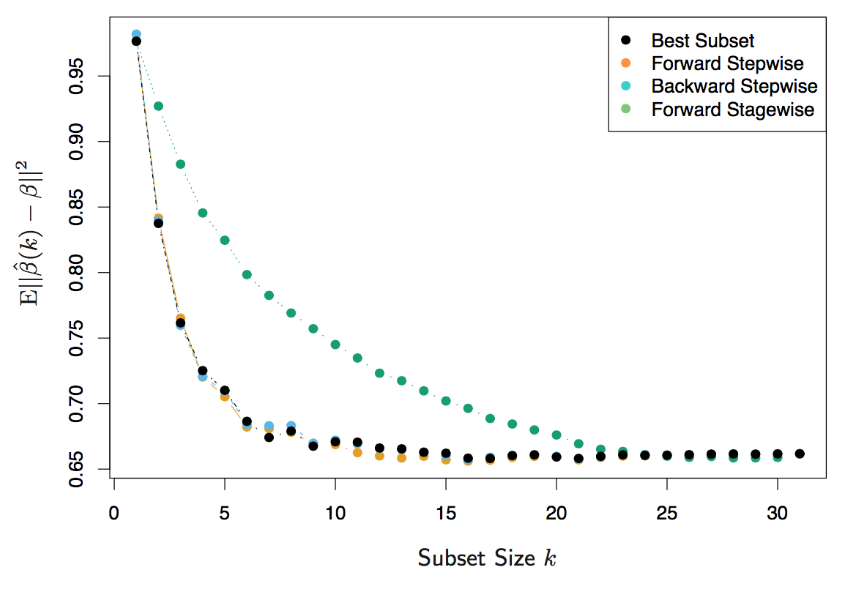
\includegraphics[width=1\textwidth]{Figure_3.PNG}
\caption{\label{fig:3}Four subset selection techniques on a simulated linear regression problem. Results are obtained by averaging errors after 50 simulations.}
\end{figure}

\end{document}